\chapter{Background}
\label{chap:bg}
In this chapter, we first introduce the generative probability topic HDP models. Subsequently, we demonstrate the Gaussian process models for regression and classification.
They are the basic of our framework.

\section{Hierarchical Bayesian Models}
\label{bg:hbm}
LDA~\cite{blei2003latent} and HDP~\cite{teh2006hdp} are generative probabilistic models and were originally proposed as hierarchical Bayesian models for natural language processing. 
In the models, each document is viewed as a bag of words. Those words that frequently co-occur in the same documents are clustered into the same topic. A document is posited to be a random mixture of latent topics and each word is assumed to be created by one of the document's topics according to its unique joint probability distribution over words. 
HDP model is a natural nonparametric generalization of LDA model. To help us better understand HDP models, we will first briefly discuss LDA models.

\subsection{LDA}
\label{bg:lda}
Different from the well-known probabilistic latent semantic analysis (pLSA), LDA model assumes that the distribution of topics has a Dirichlet prior. The standard LDA model is illustrated in Fig.~\ref{fig:lda}. The outer plate represents a corpus with $M$ documents. $N_j$ denotes the number of words in $j$th document. The meanings of each character in the graph are:

\begin{itemize}
	\item[]$\alpha$ is the parameter of the Dirichlet prior on the topic distribution in a document
	\item[]$\beta$ is the parameter of the Dirichlet prior on the word distribution in a topic
	\item[]$x_{ji}$ is the $i$th word in $j$th document
	\item[]$\theta_j$ is the topic distribution in $j$th document
	\item[]$z_{ji}$ is the topic specified for the word  $x_{ji}$
\end{itemize}

\begin{figure}[!htp]
	\centering
	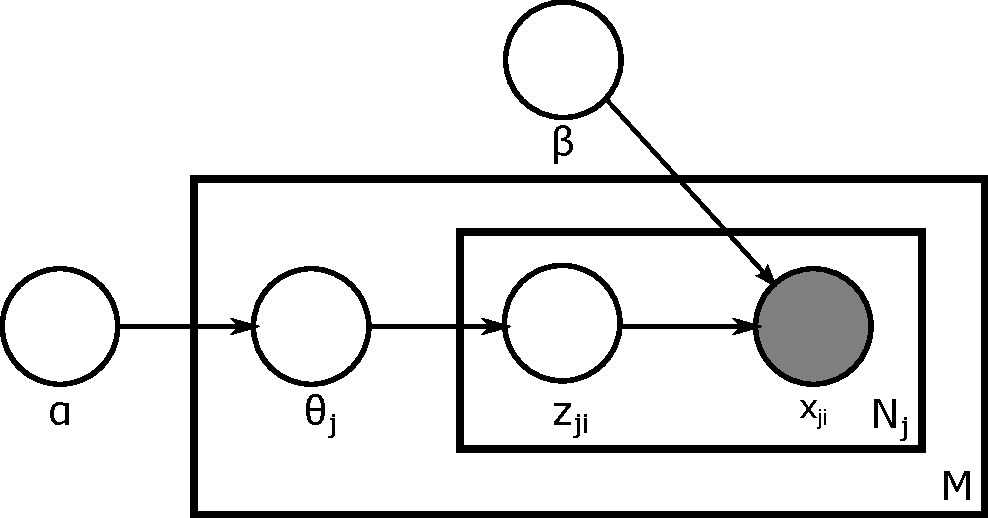
\includegraphics[width = 0.5\textwidth]{figures/Latent_Dirichlet_allocation.pdf}
	\caption[The standard graphical model representation of LDA model]
	{The standard graphical model representation of LDA model \cite{blei2003latent}. The outer plate represents the corpus with $M$ documents and the inner plate is the $j$th documents containing $N_j$ words. The words and their topics are repeatedly choice until the construction of this document is finished. The shading denotes an observation, i.e. the word. The topics are latent.}
	\label{fig:lda}
\end{figure}

In LDA model, the number of topics is manually defined in advance, and we denote it as $K$. Each topic $k$ is modeled as a multinomial distribution $\phi_k=[\phi_{ki},\cdots,\phi_{kW}]$ over a word vocabulary of size $W$. $\phi_k$ is drawn from the Dirichlet distribution $\phi_k \thicksim Dir(\beta)$. 
$\theta_j = [\theta_{j1},\cdots,\theta_{jK}]$ is the multinomial distribution over $K$ topics in $j$th document and it is drawn from the Dirichlet distribution $\theta_j \thicksim Dir(\alpha)$ and $\alpha = [\alpha_1,\cdots,\alpha_K]$.  Each word $x_{ji}$ is labeled with a topic $z_{ji}=k$ which is drawn from the multinomial distribution $z_{ji} \thicksim Multinomial(\phi_j)$. The word $x_{ji}$ is drawn from the multinomial distribution $x_{ji} \thicksim Multinomial(\beta_{z_{ji}=k})$. The joint distribution of topic mixture $\theta_j$, words $\mathbf{x}_j = \{x_{ji} \}$ and their corresponding topics $\mathbf{z}_j={z_{ji}}$ under the given the parameters $\alpha$ and $\beta$ is

\begin{equation}
	\begin{aligned}
		p(\mathbf{x}_j, \mathbf{z}_j, \theta_j|\alpha, \beta) = p(\theta_j|\alpha)\prod_{i=1}^{N_j}p(z_{ji}|\theta_j)p(x_{ji}|z_{ji}, \beta)\\
		=\frac{\Gamma(\sum_{k=1}^K \alpha_k)}{\prod_{k=1}^K \Gamma(\alpha_k)} \theta_{j1}^{\alpha_1-1}...\theta_{jK}^{\alpha_K-1}\prod_{i=1}^{N_j}\theta_{jz_{ji}}\phi_{z_{ji}x_{ji}}.
	\end{aligned}
	\label{eq:lda_joint_distri}
\end{equation}


The generation process of a corpus with $M$ documents is summarized as follows:
\begin{itemize}
	\item[1] For document $j$, a multinomial distribution over $K$ topics $\theta_j = [\theta_{j1},\cdots,\theta_{jK}]$ is generated by $Dir(\alpha)$.
	\item[2] For each topic $k$, a multinomial distribution over a word vocabulary of size $W$ $\phi_k=[\phi_{ki},\cdots,\phi_{kW}]$ is generated by $Dir(\beta)$.
	\item[3] For each words $x_{ji}$, a topic $z_{ji}=k$ is first drawn from $Multinomial(\theta_j)$, then a word is drawn from $Multinomial(\phi_k)$. This step is repeated until $N_j$ words are generated.
	\item[4] step 1 to 3 is repeated until $M$ documents are generated.
\end{itemize}

From the process we see that, the latent parameters $\theta,~\phi $ need to be inferred. The most widely adopted inference schemes include \emph{Variational inference-EM}~\cite{blei2006variational} and \emph{Gibbs Sampling}~\cite{casella1992explaining}.

We notice that, the number of topics $K$ is fixed manually beforehand. However, it is not obvious how to choose the optimal number of topics. Furthermore, in LDA model, all documents do not share the all topics. Thus, it is possible that individual topics are learned for some documents. To address these problem, HDP model is proposed.

\subsection{HDP}
\label{bg:hdp}
Teh et al.~\cite{teh2006hdp} extended LDA model to a non-parametric Bayesian approach. In contrast to LDA models, HDP models will automatically determine the number of topics.
HDP uses two \emph{Dirichlet process} Dirichlet process (DP) in two levels. The first Dirichlet process is used to capture the uncertainty in the number of topics. So a common base distribution is selected which represents the countably-infinite set of possible topics for the corpus, and then the finite distribution of topics for each document is sampled from this base distribution by the second Dirichlet process. This allows the different documents to share statistical strength.
It has the standard graphical representation as shown in Fig.~\ref{fig:hdp_graph}.

\begin{figure}[!htbp]
	\center
	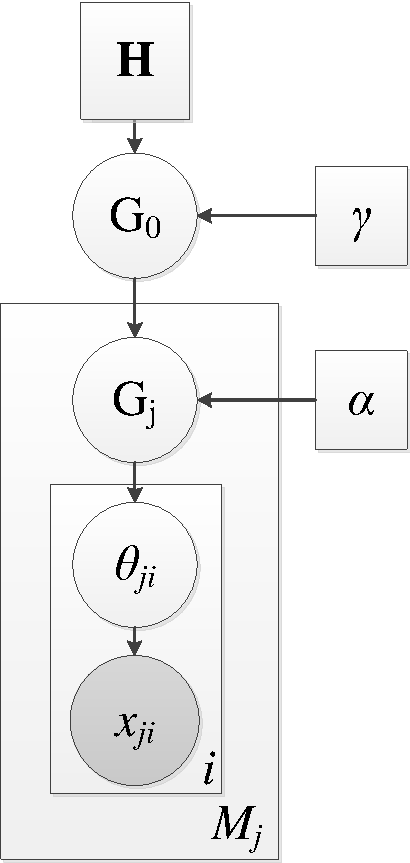
\includegraphics[width=3cm, height = 5cm]{figures/HDP_standard_graph-crop.pdf}
	\caption[The standard graphical model representation of HDP model]
	{The standard graphical model representation of HDP model~\cite{teh2006hdp}. The rectangles represent replication of the model within the rectangle. The outer plate denotes the whole corpus with $M$ documents, while the inner plate denotes the $j$th documents containing $N_j$ words. The shading denotes an observation, i.e. the word. The topics are latent.}
	\label{fig:hdp_graph}
\end{figure}

In the model, $G_0$ is the base measure with probability one and shared across all documents. It is a draw from a DP with based distribution H and concentration parameter $\gamma$,

\begin{equation*}
	G_0|\gamma,H \thicksim DP(\gamma,H).
\end{equation*}

This process can be formulated using the stick-breaking construction~\cite{teh2006hdp}:
\begin{align}
	\label{eq:g0}
	&G_0 = \sum^\infty_{k=1}\pi _k\delta_{\phi_k}\\
	\label{eq:gem1}
	where~~~~~~~~&\pi_k'\thicksim Beta(1,\lambda),~~~~~~for~~k=1,...,\infty \\
	\label{eq:gem2}
	&\pi_k =\pi _k'\prod^{k-1}_{l=1}(1-\pi _l')\\ 
	&\phi_k|\gamma,H \thicksim H
	\label{eq:phi_k}
\end{align}

This DP generates a distribution $G_0$ in the form of an infinite mixture of atoms $\phi_k$ Eq.~\eqref{eq:g0}. $\delta_{\phi_k}$ is the Delta function at support point $\phi_k$. $\{\pi_k\}$ are random probability measures (mixtures over topics) and $\Sigma_{k=1}^\infty \pi_k=1$. Its construction can be conveniently noted as $\pi_k \thicksim GEM(\gamma)$ with the definition of Eq.~\eqref{eq:gem1} and~\eqref{eq:gem2}.

From Eq.~\eqref{eq:g0} we know that drawing from the mixture $G_0$ results in one of atoms $\phi_k$. $\{\phi_k\}$ are parameters of multinomial distributions over words in vocabulary, i.e. topics. They are drawn from $H$ Eq.~\eqref{eq:phi_k}. Therefore, $H$ is interpreted as a distribution over multinomial distributions and defined as a Dirichlet distribution:

\begin{align*}
	H = Dir(D_0).
\end{align*}
Then Eq.~\eqref{eq:phi_k} can be rewritten as:
\begin{equation}
	\phi_k|\gamma,H  \thicksim Dir(D_0),
\end{equation}
where $D_0$ is the parameter for the Dirichlet distribution we have discussed in Sec.~\ref{bg:lda}.

In the second level of the model, $G_t$ is drawn from the second DP with concentration parameter $\alpha$ and based distribution $G_0$:

\begin{equation}
	G_j|\alpha,G_0 \thicksim DP(\alpha,G_0).
\end{equation}

Its stick-breaking construction is as follows:
\begin{align}
	\label{eq:gt}
	&G_j = \sum^\infty_{k=1}\pi _{jk}\delta_{\phi_k},\\
	where~~~~~~~~&\pi_{jk} =\pi _{jk}'\prod^{k-1}_{l=1}(1-\pi _{jl}'),\\
	&\pi_{jk}'\thicksim Beta(1,\alpha),\\
	&\phi_k|\alpha,G_0 \thicksim G_0.
\end{align}

%$G_0$ is itself a drawn from the first DP. Thus, $G_0$ is a prior distribution over the whole corpus and a sample $G_j$ is its subset. $G_j$ also can be expressed using the stick-breaking construction as follows:

Because $G_0$ is itself a drawn from the first DP, $G_0$ is a prior distribution over the whole corpus.
For each document $j$, $G_j$ has the same support at the same locations ${\phi_k}_{k=1}^{\infty}$ as $G_0$, i.e. all of the documents share the same set of topics. Therefore, $G_j$ is a re-weighted mixture of the atoms in $G_0$ (Eq.~\eqref{eq:gt}). 

For each word $i$ in document $t$ noted as $x_{ji}$, a topic $\theta_{ji}$ is first drawn from $G_j$. Then, the word $x_{ji}$ is drawn from the multinomial distribution $Multinomial(\phi_{\theta_{ji}})$ over words which models topic $\theta_{ji}$.
HDP model also can be inferred by \emph{Gibbs sampling} or \emph{Variational inference} schemes which is similar to LDA model.

%The same as LDA models, the latent parameters $\theta,~\phi $ need to be inferred.
%We use Gibbs sampling schemes to do inference under an HDP model, which is adopted in~\cite{teh2006hdp}.

%The hyper-parameters $\gamma$ and $\alpha$ are empirically predefined. They are priors on the concentration of the word distribution within topics. They influence the the number of activities in $G_0$ and $G_j$. The parameter $D_0$ for the Dirichlet distribution is also set empirically.


%******************************************************************************
\section{Gaussian Process Models}
\label{bg:gp}
In the last decades, there have been numerous studies in non-parametric Bayesian approaches based on Gaussian process to be applied in supervised learning problems~\cite{rasmussen2006gaussian}. 
In comparison with parametric approaches, the prior is directly defined as a Gaussian distribution and learned from the training dataset, instead of defining prior distributions over parameters of a learning machine (such as weights and biases in case of a neural net).  Gaussian Process models are kernel-based methods, they can be optimized exactly, given the values of their hyper-parameters (such as the length-scale of a Gaussian kernel), and this often allows a fine and precise trade-off between fitting the data and smoothing. 
In addition, Gaussian process models make probabilistic (Gaussian) prediction so that one can compute empirical confidence intervals and exceeding probabilities that might be used to refit (online fitting, adaptive fitting) the prediction in some region of interest. 
This property is crucial for tasks of abnormal events detection.

Supervised learning problems have two domains. The first one is regression of which the output is the prediction of continuous quantities. The second is classification. Its outputs are discrete class labels. In this section, we will briefly introduce how Gaussian process models are applied for regression and classification problems. 

\subsection{Gaussian Process for Regression}
\label{bg:gpr}
Assumes that, we have a training dataset of n observations, $\mathcal{D}=\{(\mathbf{x}_i,y_i)| i=1,...,n\}$. $\mathbf{x}$ denotes an input feature vector of dimension $D$ and $y$ is its corresponding target value. A latent function $f(\mathbf{x})$ relates $\mathbf{x}$ and $y$ as follows:
\begin{equation}
	y = f(\mathbf{x})+\varepsilon,
\end{equation}
where $\varepsilon$ is a mean zero Gaussian noise, $\varepsilon \thicksim \mathcal{N}(0,\sigma_n^2)$. Our task is to uncover the latent functional relationship $f(\mathbf{x})$ from the training dataset and make a prediction of value $y'$ for a new input feature vector $\mathbf{x}'$. This is a general Bayesian regression problem. For example, as shown in Fig.~\ref{fig:gpr_eg_a}.

\begin{figure}
	\centering
	\subfigure[Training dataset with six noisy data points]{
		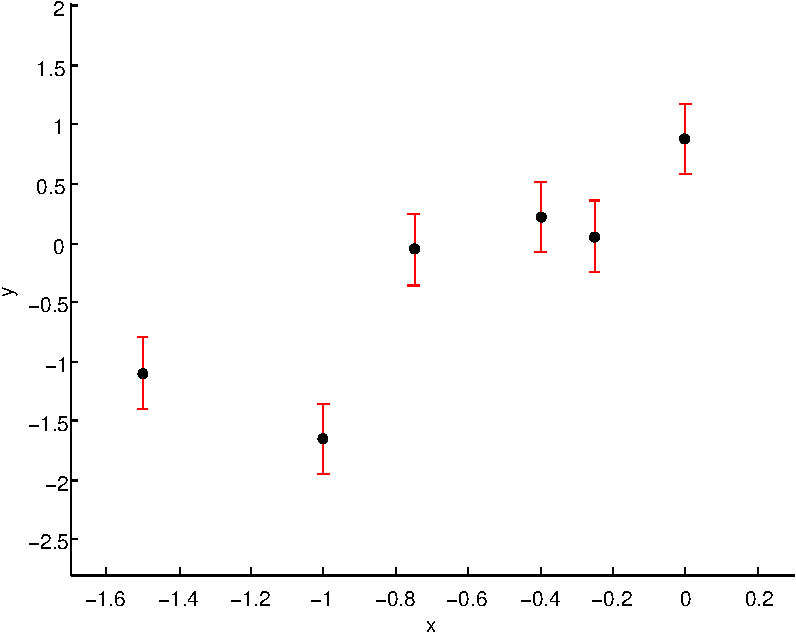
\includegraphics[width = 0.4\textwidth]{figures/gp/gpr_eg-crop.pdf}
		\label{fig:gpr_eg_a}
	}
	\hspace{1cm}
	\subfigure[Prediction for x=0.2]{
		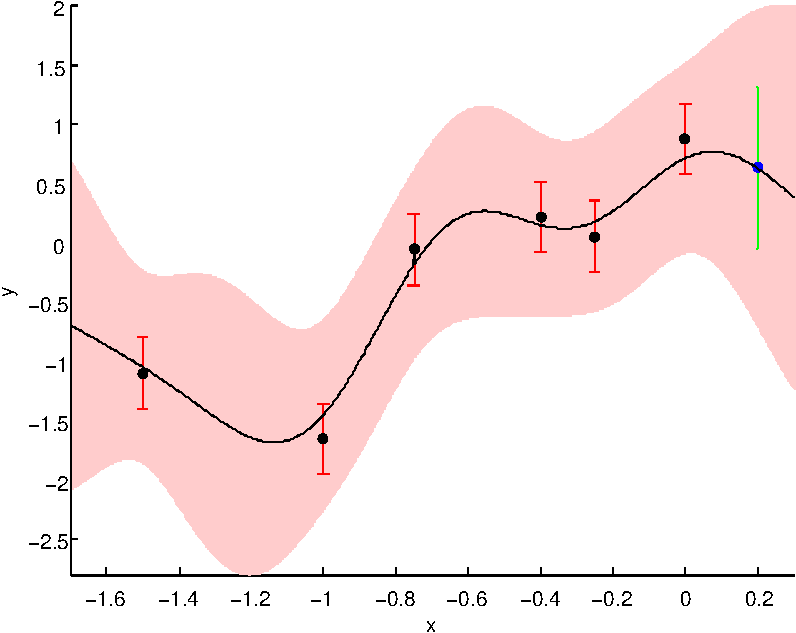
\includegraphics[width = 0.4\textwidth]{figures/gp/gpr_eg_result-crop.pdf}
		\label{fig:gpr_eg_b}
	}
	\caption[An example for GP regression]
	{An example for GP regression. (a) Given six six noisy data points . (b) Prediction of GP regression model at test point $x_*=0.2$. The red area represent the pointwise 95\% confidence area for the underlying function $f$. In both plots, the Vertical lines indicate the error bars.}
\end{figure}

In GP models, the prior distribution of $f(\mathbf{x})$ is assumed as a Gaussian process.
\begin{equation}
	f(\mathbf{x}) \sim \mathcal{GP}(m(\mathbf{x}),k(\mathbf{x},\mathbf{x}'))
	\label{eq:gp_prior}
\end{equation}

Gaussian process can be defined as a collection of random variables, any finite number of which have a joint Gaussian distribution. It is completely specified by of mean function and covariance function as:

\begin{equation*}
	\begin{aligned}
		m(\mathbf{x}) &= \mathbb{E}[f(\mathbf{x})],\\
		k(\mathbf{x},\mathbf{x}') &= \mathbb{E}[(f(\mathbf{x})-m(\mathbf{x}))(f(\mathbf{x}')-m(\mathbf{x}'))]
	\end{aligned}
\end{equation*}

Without the loss of generality, the mean function will be assumed as zeros hereafter. Therefore, the GP prior in Eq.~\eqref{eq:gp_prior} only depends on the convariance function:
\begin{equation}
	cov(\mathbf{x},\mathbf{x}')=k(\mathbf{x},\mathbf{x}') = \mathbb{E}[f(\mathbf{x})f(\mathbf{x}')]
\end{equation}
The convariance function is also well-known as kernel function. We will discuss in detail it later in this section. Here, we adopt the Gaussian kernel as an example:

\begin{equation}
	k(\mathbf{x}_i,\mathbf{x}_j) = exp(-\frac{1}{2}|\mathbf{x}_i-\mathbf{x}_j|^2)
	\label{eq:se}
\end{equation}
For hereafter convenient discussion, we denote some impotent expression of convariance matrix. The training dataset are denoted as $\mathbf{X} = [\mathbf{x}_1,...,\mathbf{x}_n]$ and $\mathbf{y} = [y_1,...,y_n]$. $\mathbf{x}_*$ is a single test point. $K = K(\mathbf{X},\mathbf{X})$ is a $n\times n$ covariance matrix between $n$ training points. $\mathbf{k}_*= K(\mathbf{X},\mathbf{x}_*)$ is a covariance vector between $n$ training points and the test point. $k(\mathbf{x}^*\mathbf{,x}^*)$ is covariance for test point. All entries of these convariance matrix are computed by kernel function such as Eq.\ref{eq:se}.

\begin{figure}[!htbp]
	\centering
	\subfigure[$\ell= 1.0$]{
		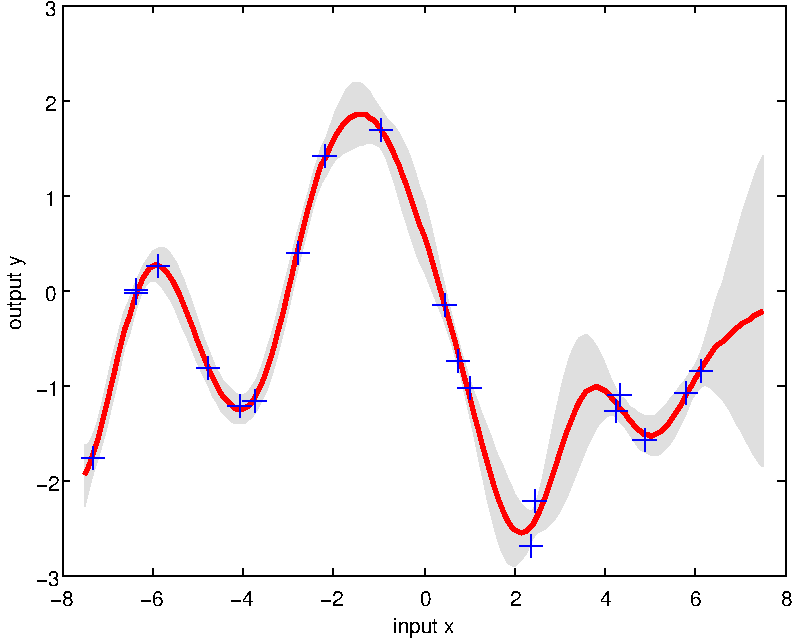
\includegraphics[width = 0.4\textwidth]{figures/gp/gpr_parameter_exsample1-crop.pdf}
		\label{fig:gpr_l_1}
	}\\
	\subfigure[$\ell= 0.3$]{
		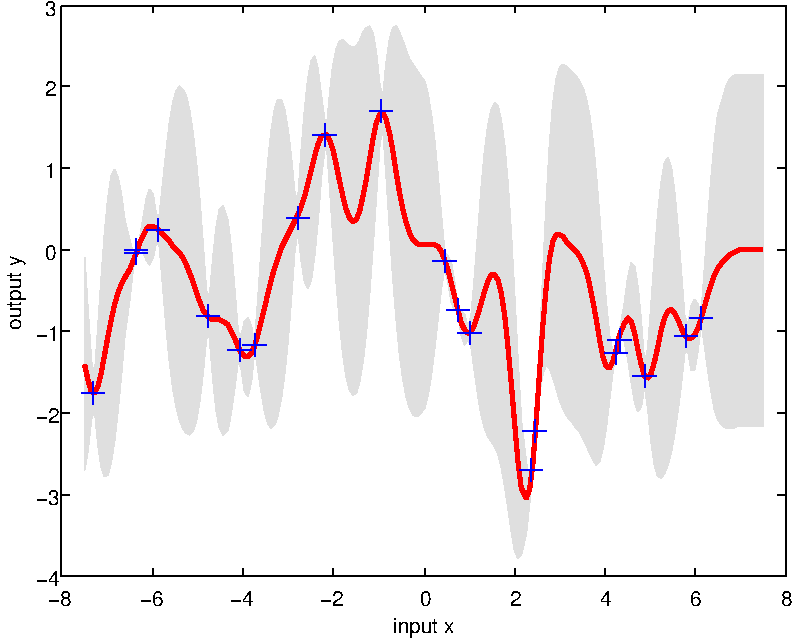
\includegraphics[width = 0.4\textwidth]{figures/gp/gpr_parameter_exsample2-crop.pdf}
		\label{fig:gpr_l_2}
	}
	\hspace{1cm}
	\subfigure[$\ell= 3.0$]{
		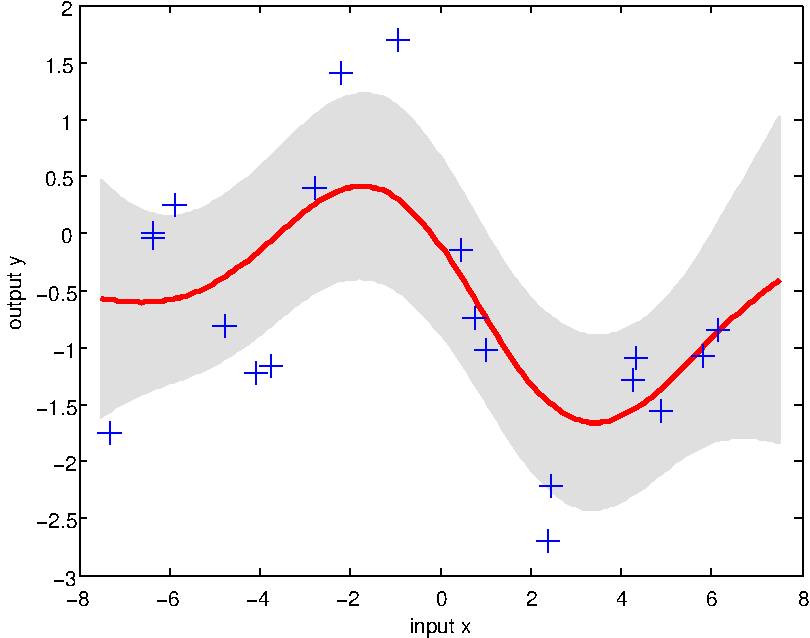
\includegraphics[width = 0.4\textwidth]{figures/gp/gpr_parameter_exsample3-crop.pdf}
		\label{fig:gpr_l_3}
	}
	\caption[The effect of haperparameter on GP regression]
	{20 simulated data points are randomly generated from a GP with the Gaussian kernel with hyper-parameters $(\ell, \sigma_f,\sigma_n)=(1,1,0.1)$ , as noted by the blue + symbols. Using Gaussian process regression, 200 points which uniformly range between $[-7.5,~7.5]$ are predicted with different hyper-parameters. The red line represents the regression results and the gray area regression the 95\% confidence region for the underlying function $f$. The hyper-parameters are (a) $(1,1,0.1)$, (b) $(0.3,1.08,0.00005)$ and (c) $(3.0,1.16,0.89)$  respectively.}
	\label{fig:gpr_l}
\end{figure} 

According to the assumption in GP model, the joint distribution of the observed target values and the function value at the test location has the prior:

\begin{equation}
	\begin{bmatrix}
		\mathbf{y}\\
		f_*
	\end{bmatrix}
	\sim \mathcal{N} \begin{pmatrix}
		\mathbf{0} & \begin{bmatrix}
			K + \sigma_n^2 \mathbf{I} & \mathbf{k}_*\\
			\mathbf{k}_*              & k(\mathbf{x}_*\mathbf{,x}_*)
		\end{bmatrix}
	\end{pmatrix}.
	\label{eq:joint_dist_prior}
\end{equation}
Then, the key predictive equations for Gaussian process regression are derived~\cite{williams1996gaussian}:
\begin{align}
	f_*|\mathbf{X},\mathbf{y},\mathbf{x}_* &\sim \mathcal{N}(\bar{f}_*,\mathbb{V}(f_*)),\label{eq:gpr_prediction}\\
	\bar{f}_* &\triangleq \mathbf{k}_*^T (K-\sigma_n^2 \mathbf{I})^{-1} \mathbf{y},\\
	\mathbb{V}(f_*) &= k(\mathbf{x}_*\mathbf{,x}_*)-\mathbf{k}_*^T(K+\sigma_n^2 \mathbf{I})^{-1}\mathbf{k}_*
\end{align}
Fig.~\ref{fig:gpr_eg_b} show an example of prediction at test location $x_*=0.2$ with Gaussian process regression given six noisy data points.


From above discussion, we have seen that the covariance function is the crucial ingredient in Gaussian process predictor. It encodes our assumptions about the function $f(\mathbf{x})$ which we wish to learn. Under the Gaussian process view, the nearness or similarity between two points are defined by the covariance function.

Several kernel functions such as polynomial kernel have been successfully applied to machine learning. The Gaussian kernel which is also called as radial basis function (RBF), is one of the most widely used kernels since its robustness for different types of data. Its standard expression is:
\begin{equation}
	k_{RBF}(\mathbf{x}_i\mathbf{,x}_j) = \sigma^2 exp(-\frac{\left.\|\mathbf{x}_i - \mathbf{x}_j\right.\| ^2}{2\ell^2}).
	\label{eq:rbf}
\end{equation}

$\Theta = [\sigma,\ell]$ is the hyper-parameter set for RBF, of which $\ell$ in the function is
the characteristic length-scale, which informally can be roughly considered as the distance you
have to move in input space for the function value to become uncorrelated. The smaller $\ell$ we choose, the more rapidly the function varies. In this case, all of the training points are more correctly classified.  Fig.~\ref{fig:gpr_l} illustrates the influence of the hyper-parameters on the results of Gaussian process regression.
% explain?

Moreover, if the length-scale $\ell$ varies with input dimensions, e.g.~$\mathbf{\ell} = [\ell_1,\ldots,\ell_d]$, there is another kernel called the Automatic Relevance Determination (ARD) which is derived form RBF:
\begin{equation}
	k_{ARD}(\mathbf{x}_i\mathbf{,x}_j) = \sigma^2 exp(-\sum\limits_{b=1\ldots d}\frac{\left.\|{x_i^b - x_j^b}\right.\| ^2}{2\ell_b^2}).
	\label{eq:ard}
\end{equation}
$x_i^b$ indicates the $b$th dimension value of the $i$th input point. The ARD kernel has been proved to be an effective kernel successfully removing irrelevant information~\cite{williams1996gaussian}. It provides a parametrization scheme for automatic feature reduction especially for the high-dimensional challenge.

\subsection{Gaussian Process for Classification}
\label{bg:gpc}
Different from regression problems, the output of classification are discrete class labels.
The training set need to be redefined as $(\mathbf{X},\mathbf{y})=\{\mathbf{x}_i,y_i)| i=1,...,n\}$. $y_i$ is the corresponding class label for input vector $\mathbf{x}_i$. The task is labeling a new test point $\mathbf{x}_*$ to a class $y_*$. For simple illustrating the binary classification with target $y_i \in \{-1,+1\}$ is considered here. The binary classification is easily extended to multiple classification by using the one-against-all or one-against-one strategy. 

Gaussian process models generate a discrete label $y_i$ for a data point $\mathbf{x}_i$ via a continuous latent variable $f_i$. A likelihood model $p(\mathbf{y}|\mathbf{f})$ characterizes the monotonic relationship between latent variable $\mathbf{f}$ and the probably observed annotation $\mathbf{y}$. The logistic and probit function are the most common choices. Specially, the probit function is simply the standard normal cumulative distribution function. Their forms are
\begin{align}
	\varphi_{logit}(z) &= \frac{1}{1+e^{-z}},\\
	\varphi_{probit}(z) &= \int_{-\infty}^z \frac{1}{\sqrt{2\pi}} exp(-\frac{x^2}{2}) dx.
\end{align}
Then, the likelihood term becomes
\begin{equation}
	p(y_i=+1|f_i) = \varphi (y_i f_i).
\end{equation}

To make a probability prediction for the label of test point $\mathbf{x}_*$, the distribution of the latent variable $f_*$ corresponding to test point $\mathbf{x}_*$ need to be computed first~\cite{rasmussen2006gaussian}
\begin{equation}
	p(f_*|\mathbf{X},\mathbf{y},\mathbf{x}_*) = \int p(f_*|\mathbf{X},\mathbf{x}_*,\mathbf{f}) p(\mathbf{f}|\mathbf{X},\mathbf{y})d\mathbf{f},\label{eq:gpc_posterior}
\end{equation}
where $p(f|\mathbf{X},\mathbf{y}) = p(\mathbf{y}|\mathbf{f})p(\mathbf{f}|\mathbf{X})/p(\mathbf{y}|\mathbf{X})$ is the posterior over latent variables $\mathbf{f} = (f_1,\ldots,f_n)$, which are the latent variables corresponding to training set $(\mathbf{X},\mathbf{y})$. Subsequently, we use this distribution over the latent variable $f_*$ to make a probabilistic prediction~\cite{rasmussen2006gaussian}
\begin{equation}
	p(y_*=+1|\mathbf{X},\mathbf{y},\mathbf{x}_*) = \int p(y_*|f_*)p(f_*|\mathbf{X},\mathbf{y},\mathbf{x}_*) df_* .\label{eq:gpc}
\end{equation}

The posterior $p(\mathbf{f}|\mathbf{X},\mathbf{y})$ in Eq.~\eqref{eq:gpc_posterior} is non-Gaussian likelihood. Therefore, the integral is analytically intractable. Similarly, Eq.\ref{eq:gpc} might be also analytically intractable for certain sigmoid functions. To solve this problem, a number of approximations have been suggested. The \emph{Monte Carlo Markov Chain} (MCMC) sampling is a standard procedure for posterior inference, but it is computation expensive. Under Gaussian process models, two analytic approximation approaches are commonly applied: \emph{Laplace's } approximation method (LP) \cite{williams1998bayesian} and \emph{expectation propagation} (EP) algorithm \cite{minka2001family}. They both approximate the non-Gaussian joint posterior with a Gaussian one. In this thesis, the LP method will be adopted because of its less computation and easier inference. Interested readers are referred to \cite{rasmussen2006gaussian} for more details on the two methods.

Laplace's method approximate the posterior $p(\mathbf{f}|\mathbf{X},\mathbf{y})$ using a Gaussian distribution:
%\begin{equation}
%q(\mathbf{f}|\mathbf{X},\mathbf{y}) = \mathcal{N}(\mathbf{f}|\hat{\mathbf{f}},A^{-1}),
%\end{equation}
\begin{equation}
	q(\mathbf{f}|\mathbf{X},\mathbf{y}) = \mathcal{N}(\hat{\mathbf{f}},(K^{-1}+W)^{-1}),
\end{equation}
where $\hat{\mathbf{f}}=argmax_\mathbf{f} p(\mathbf{f}|\mathbf{X},\mathbf{y})$ and $W \triangleq -\bigtriangledown\bigtriangledown log~p(\mathbf{y}|\mathbf{f})$ is diagonal.
%$A = -\bigtriangledown\bigtriangledown log p(\mathbf{f}|\mathbf{X},\mathbf{y})|_{\mathbf{f}=\hat{\mathbf{f}}}$ is the Hessian of negative log posterior at the point.

Then, the posterior for latent $f_*$ in Eq.~\eqref{eq:gpc_posterior} is approximated as a Gaussian
\begin{align}
	q(f_*|\mathbf{X},\mathbf{y},\mathbf{x}_*) &= \mathcal{N}(\mathbb{E}[f_*|\mathbf{X},\mathbf{y},\mathbf{x}_*],\mathbb{V}[f_*|\mathbf{X},\mathbf{y},\mathbf{x}_*]),\\
	with~~~~~~~~~~~~\mathbb{E}_q[f_*|\mathbf{X},\mathbf{y}] &= \mathbf{k}_*^T K^{-1} \hat{\mathbf{f}} = \mathbf{k}_*^T \bigtriangledown log~p(\mathbf{y}|\hat{\mathbf{f}}) ,\\
	\mathbb{V}_q[f_*|\mathbf{X},\mathbf{y},\mathbf{x}_*] &= k(\mathbf{x}_*\mathbf{,x}_*)-\mathbf{k}_*^T(K+W^{-1})^{-1}\mathbf{k}_*.
\end{align}

With the mean and variance of $f_*$, the predictions in Eq.~\eqref{eq:gpc} is computed as 

\begin{equation}
	p(y_*=+1|\mathbf{X},\mathbf{y},\mathbf{x}_*) = \int \varphi(f_*)q(f_*|\mathbf{X},\mathbf{y},\mathbf{x}_*) df_* .\label{eq:gpc_lp}
\end{equation}

Notice that, if the sigmoid function is cumulative Gaussian function, Eq.~\eqref{eq:gpc_lp} can be computed analytically. Therefore, the cumulative Gaussian function will be considered in our thesis for convenient computation. 

